% !TeX spellcheck = ru_RU
% !TEX root = vkr.tex

\section{Обзор}
\label{sec:related}
% \label{sec:relatedworks}

% В данном разделе нужно описать всё, что необходимо для понимания Вашей работы и что придумали не Вы.
% В дальнейших разделах нельзя прерывать повествование, например, для рассказа о деталях используемой технологии или архитектуре старой системы, потому что читателю будет трудно отличить Ваш вклад от не Вашего.

% Любой обзор пишется с какой-то целью (обосновать актуальность, найти и описать интересные решения, сравнить и выбрать технологии) и по какой-то методике поиска материала (например, поиск N релевантных статей на таких-то сервисах).
% Не будет лишним это всё явно описать.

В этом разделе будут описаны существующие решения, разобраны модели, используемые в работе,
а также алгоритмы отслеживания траекторий на видео.

\subsection{Обзор существующих решений}

Идея данной работы не уникальна. Существует множество реализаций, предназначенных для разных целей.
Большинство сложных и качественных систем делается на заказ для компаний,
поэтому к ним нет открытого доступа.
Ниже будет сравнение нескольких открытых реализаций, решающих похожую задачу.
Все работы ниже достойны внимания, но каждую реализацию стоит выбирать конкретно под свой проект.

\begin{itemize}
    \item \texttt{Equipment Utilization and Activity Classification}\footnote{Ссылка на репозиторий с работой: \url{https://github.com/samir-m0hamed/Equipment-Utilization-and-Activity-Classification}.}:
    система для анализа видео, которая способна классифицировать действия строительной техники на объекте,
    а именно: простой, загрузку и разгрузку, движение и ожидание. После этого система собирает статистику,
    которая доступна в пользовательском интерфейсе.
    В этой работе реализована важная для многих компаний система, подсчитывающая время простоя каждой единицы техники,
    но есть несколько отличий от текущей работы: во-первых, это лишь модуль с обработкой,
    он принимает путь к сохранённому файлу и не делает рассылку, только обработку,
    из-за этого у пользователя могут возникнуть трудности в развёртывании,
    во-вторых, система не отслеживает статистику по людям, что также важно для компаний,
    а в-третьих, для качественной работы системы требуется камера с хорошим разрешением и без слепых зон,
    что часто является большой проблемой на строительных объектах.

    \item \texttt{Worker Safety Twin}\footnote{Ссылка на репозиторий с работой: \url{https://github.com/almosenja/Worker-Safety-Twin?utm_source=chatgpt.com}.}:
    система, способная распознавать людей и отображать их в 3D-объекте, что также позволяет отслеживать траектории рабочих в течение дня.
    Этот проект частично похож на задачу, которую будет решать предложенная в этой работе система,
    но цель этой работы --- отрисовать траектории работников для дальнейшего анализа,
    а не анализировать ситуацию в общем без привязки к конкретным людям,
    что делает требования к видеокамерам значительно выше, а также требует их большего количества.

    \item \texttt{SiteWatch}\footnote{Ссылка на репозиторий с работой: \url{https://github.com/AitchEm-bot/sitewatch?utm_source=chatgpt.com}.}:
    Этот проект больше про безопасность на объекте: он анализирует видео и проверяет наличие касок,
    находит случаи, когда возникают опасные ситуации, но не собирает статистику о работе.

\end{itemize}

Существует действительно много реализаций похожих задач, которые анализируют видео и собирают статистику,
но все они используются в разных сценариях.
В данной работе будет создана система именно для отслеживания количества персонала и техники
на строительном объекте в течение дня.

% \emph{Обзор существующих решений должен быть.}
% Здесь нужно писать, что индустрия и наука уже сделали по вашей теме.
% Он нужен, чтобы Вы случайно не изобрели какой-нибудь велосипед.

% По-английски называется related works или previous works.

% Если Ваша работа является развитием предыдущей и плохо понима\-ема без неё, то обзор должен идти в начале.
% Если же Вы решаете некоторую задачу новым интересным способом, то если поставить обзор в начале, то читатель может устать, пока доберется до вашего решения.
% В этом случае уместней поставить обзор после описания Вашего подхода к проблеме%
% \footnote{Такой подход рекомендуется в работе~\cite{SPJGreatPaper}.
%     Вполне возможно, что Ваш реальный научный руководитель будет не согласен, и потребует, чтобы обзор был в начале.}.

% В обзоре вам нужно рассказать про \emph{преимущества и недостатки} того, что было сделано до Вас.
% Неправильным будет перечислять только недостатки, так как если Ваша работа хоть где-то хуже предыдущей, то рецензент будет радостно потирать руки и заваливать Вашу работу.
% Гораздо лучше, если Вы честно признаетесь в этом сами.

% \subsection{Обзор используемых технологий}

% Для технических работ обзор может обозревать продукт, в рамках которого Вы выполняете задачу, другие продукты, где решалась схожая задача, а также используемые технологии с обоснованием выбора тех, которые Вы дальше используете.
% Это всё, скорее всего, будет отдельными подразделами обзора.
% \enquote{Выбор} подразумевает наличие вариантов, поэтому опишите, из чего выбирали и почему выбрали то, что выбрали.
% Очень желательны чёткие критерии сравнения и сводная таблица в конце, где стоят плюсы и минусы рядом с каждым рассматриваемым вариантом.

% В обзоре необходимо ссылаться на работы других людей.
% В данном шаблоне задумано, что литература будет указываться в файле \verb=vkr.bib=.
% В нём указываются пункты литературы в формате \BibTeX{}, а затем на них можно ссылаться с помощью \verb=\cite{...}=.
% Та литература, на которую Вы сошлетесь, попадет в список литературы в конце документа.
% Если не сошлетесь~---  не попадёт.
% Спецификацию в формате \BibTeX{} почти никогда (для второго курса~--- никогда), не нужно придумывать руками.
% Правильно: находить в интернете описание цитируемой статьи%
% \footnote{Например, \url{https://dl.acm.org/doi/10.1145/3408995} (дата обращения: \DTMdate{2022-12-17}).},
% копировать цитату с помощью кнопки \foreignquote{english}{Export Citation} и вставлять в \BibTeX{} файл.
% Так же умеет генерировать \BibTeX{}-описания и Google Scholar%
% \footnote{Поисковая система для научных текстов Google Scholar, \url{https://scholar.google.com} (дата обращения: \DTMdate{2024-01-13})}.
% Если так не делать, то оформление литературы будет обрастать ошибками.
% Например, \BibTeX{} по особенному обрабатывает точ\-ки, запятые и \verb=and= в списке авторов, что позволяет ему самому понимать, сколько авторов у статьи, и что там фамилия, что~--- имя, а что~--- отчество.
% Google Scholar пытается генерировать описания автоматически, так что, возможно, потребуется ручная правка~--- обязательно проверьте свой список литературы.

% В обзоре и в остальном тексте вы наверняка будете использовать названия продуктов или языков программирования (например, \csharp{}).
% Для них рекоменду\-ется (в файле \verb=preamble2.tex=) за\-дать специальные команды, чтобы писать сложные названия правильно и одинаково по всему доку\-менту.
% Написать с ошибкой  название любимого языка программирова\-ния науч\-ного руко\-водителя~--- идеальный вариант его разозлить.

\subsection{Обзор моделей семейства Ultralytics}

В работе использовались две модели из семейства \texttt{Ultralytics}~\footnote{Документация \texttt{Ultralytics}: \url{https://docs.ultralytics.com/} (дата обращения: \DTMdate{2026-09-25}).}:
\texttt{YOLO}~\cite{redmon2016yolo} и \texttt{RT-DETR}~\cite{zhao2024rtdetr}.
Обе модели изначально обучены для решения задачи детекции, но их также можно использовать для других задач.

\subsubsection{Обзор модели YOLO}

Модель \texttt{YOLO} (\texttt{You Only Look Once}) на момент выхода была революционной,
так как до этого задачу детекции решали другие модели, например, модели семейства \texttt{R-CNN}~\cite{girshick2014rcnn}.
Они решали задачу посредством поиска кандидатов, а потом из каждого кандидата извлекали признаки и делали классификацию.
Такой подход называется двустадийным, и он был медленным.
\texttt{YOLO} же решила перейти к одностадийному варианту, где рамки для объектов предсказывались сразу.
Это ускорило решение задачи детекции в десятки раз, а точность такой детекции была немного ниже,
но в то время это считалось отличным результатом.

\begin{figure}[H]
    \centering
    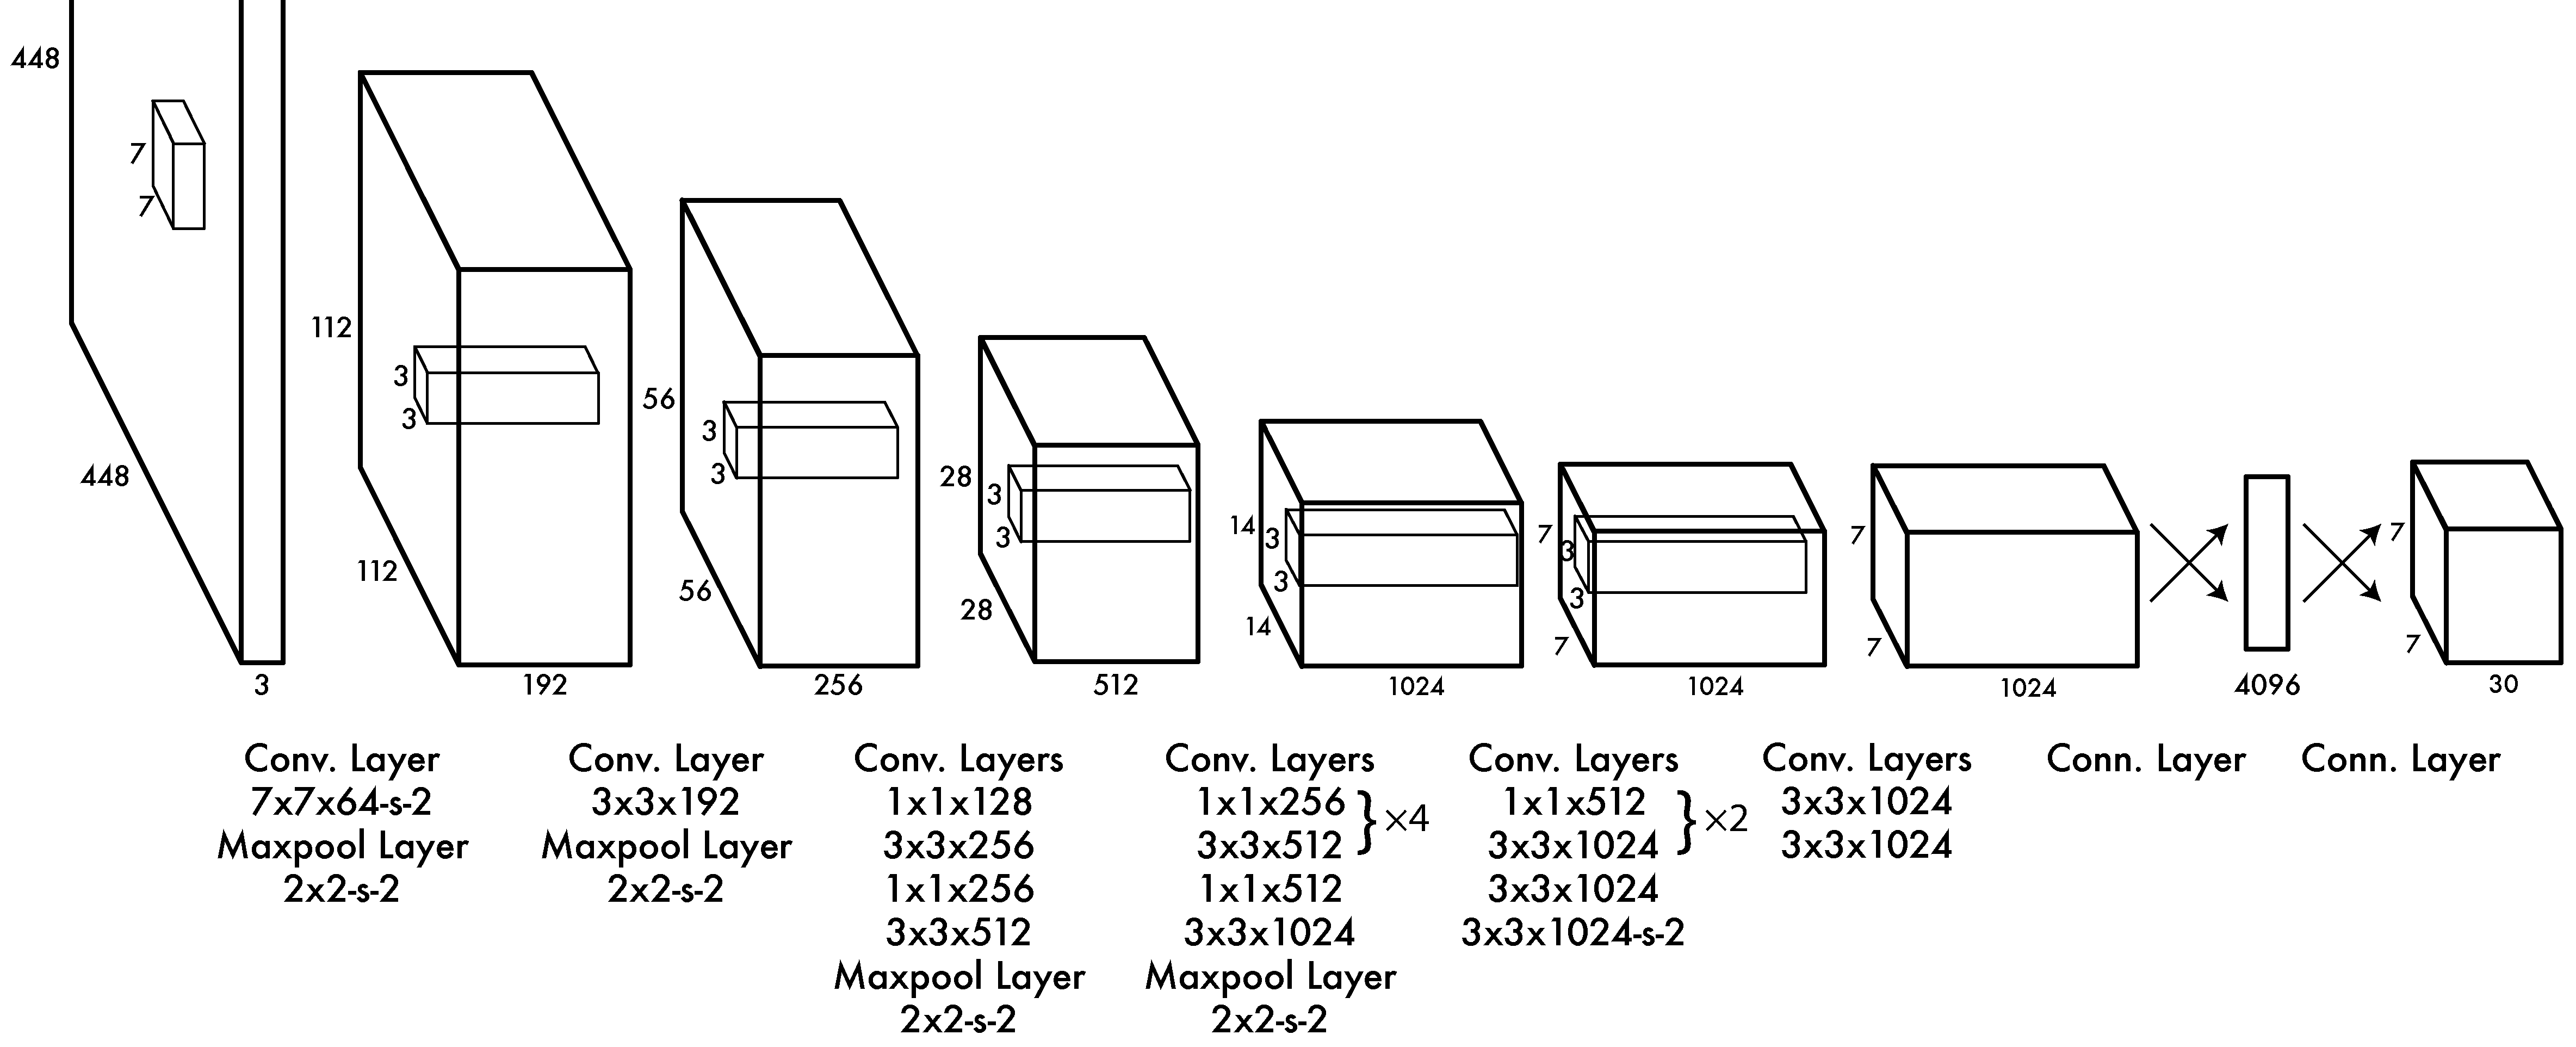
\includegraphics[page=1,width=\textwidth]{figures/yolo_v1_architecture.pdf}
    \caption{Архитектура YOLO}
    \label{fig:yolo-v1-architecture}
\end{figure}

За основу была взята архитектура \texttt{GoogLeNet}~\cite{szegedy2015googlenet}, представляющая собой обычную свёрточную сеть, в которой были заменены последние слои
для предсказания рамок, вероятностей класса и уверенности модели в том, что в рамке находится объект.
После этого специальным алгоритмом \texttt{Non-Maximum Suppression} отбирались лучшие кандидаты.

В настоящее время модели \texttt{YOLO} остаются в списке лучших для решения задачи детекции и часто являются отличным \texttt{baseline},
а после дообучения и других модификиций остаются в итоговом результате.

\subsubsection{Обзор модели RT-DETR}

Модель \texttt{RT-DETR} (\texttt{Real-Time DEtection TRansformer}) --- версия модели \texttt{DETR},
предназначенная для работы в режиме \texttt{real-time}. После выхода \texttt{ViT}~\cite{dosovitskiy2021vit} (\texttt{Vision Transformer}) --- трансформерной модели для изображений --- создание трансформер-модели для задачи детекции было лишь вопрос времени.
Трансформерная архитектура показывала \texttt{SOTA} результаты практически во всех задачах, поэтому её старались применить и для других задач.

Архитектура \texttt{DETR}~\cite{carion2020detr} использует в \texttt{encoder} части идею \texttt{ViT},
которая кодирует участки изображения в векторы.
Затем вычисляется \texttt{self-attention} между обучаемыми векторами запросов,
а затем --- \texttt{cross-attention} между выходом \texttt{self-attention} и векторами изображения.
После N таких слоёв применяются полносвязные слои и выполняется предсказание.

\begin{figure}[H]
    \centering
    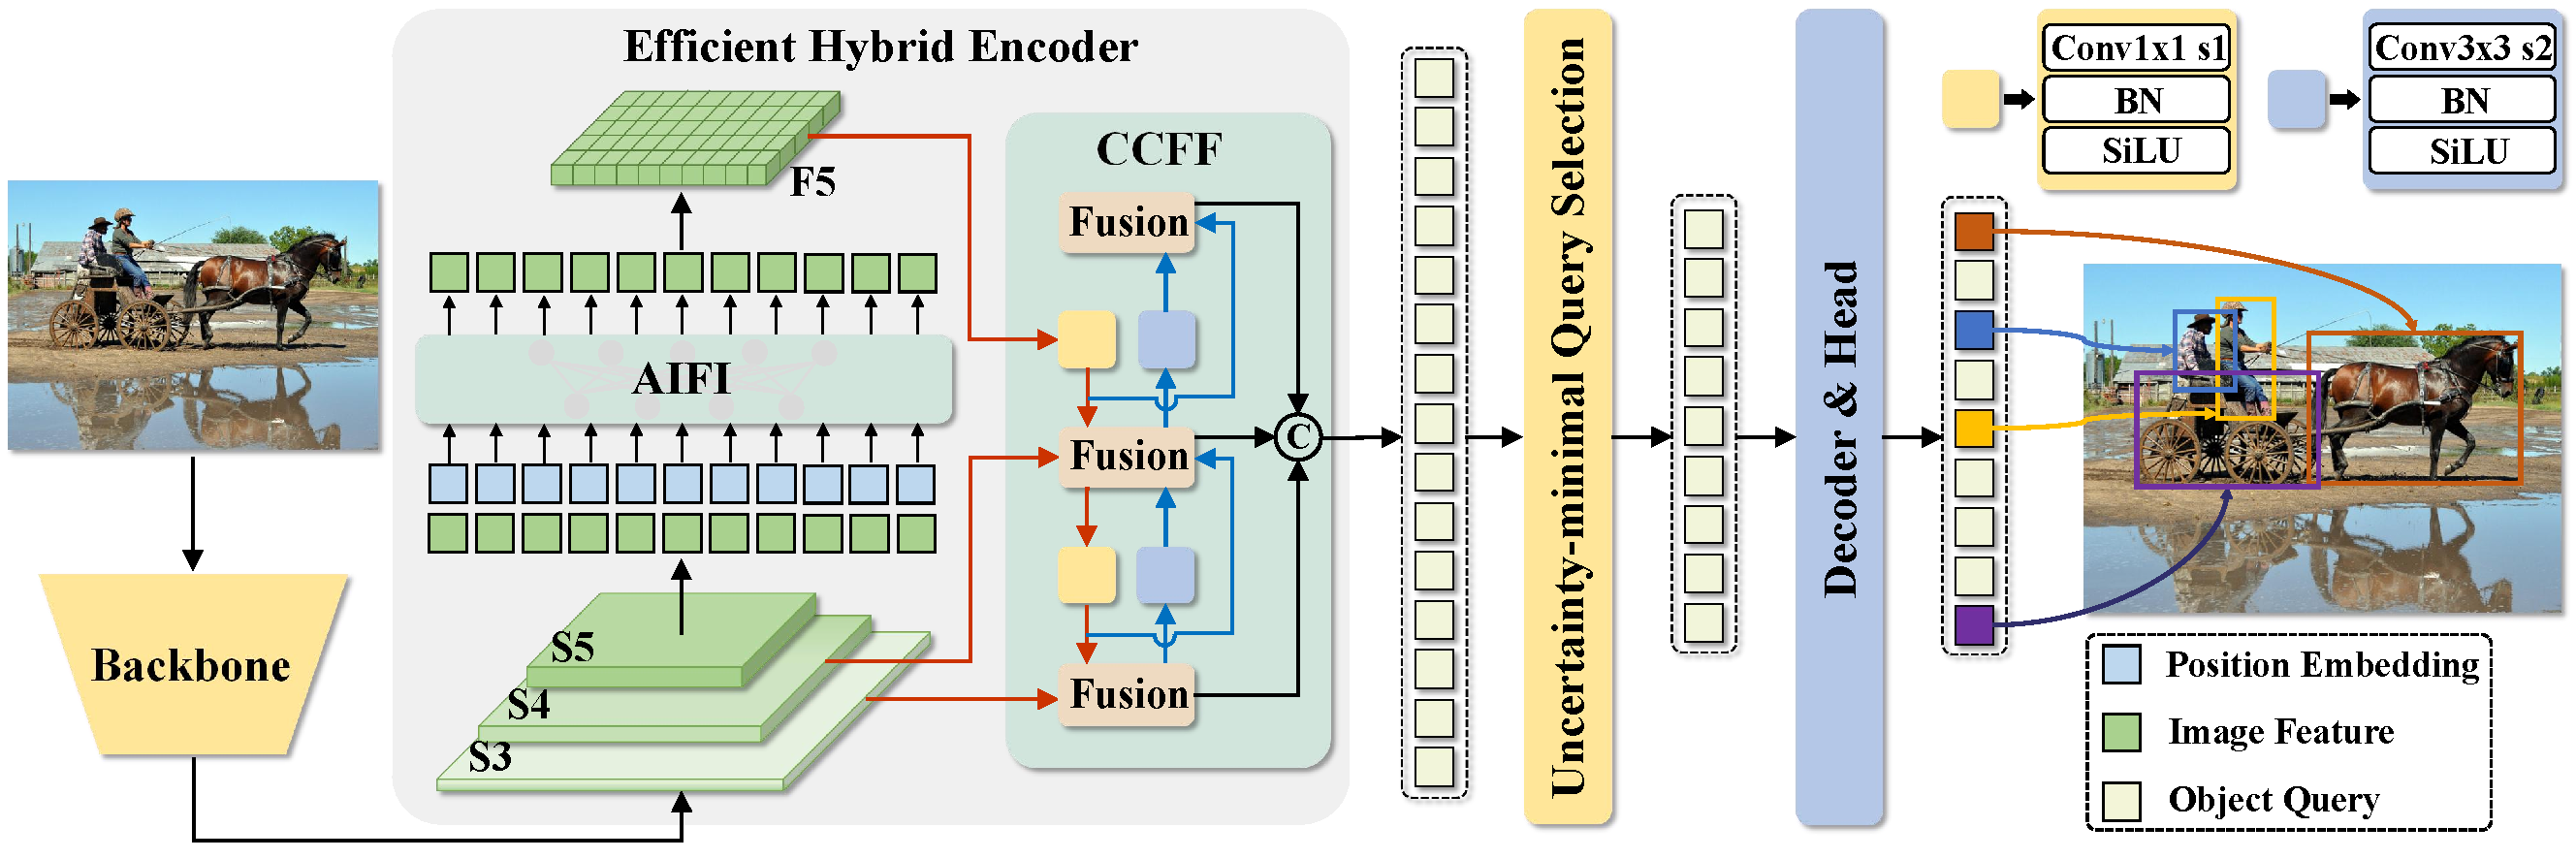
\includegraphics[width=\textwidth]{figures/rtdetr_architecture.pdf}
    \caption{Архитектура RT-DETR}
    \label{fig:rtdetr-architecture}
\end{figure}

В версии \texttt{real-time} архитектура немного изменена. В ней используется \texttt{Efficient Hybrid Encoder}, который позволяет применять различные способы агрегации векторов на разных уровнях детализации,
вместо применения \texttt{self-attention} для каждого вектора.
Для объединения мелких деталей используется \texttt{self-attention}, а для средних --- свёртки \texttt{1x1}.

Также в версии \texttt{real-time} модифицирован \texttt{decoder}: вместо выполнения сложных вычислений \texttt{self-attention} и \texttt{cross-attention} для каждого обученного вектора-запроса после извлечения признаков рассчитываются предварительные предсказания, затем отбираются только уверенные предсказания.
Есть ещё несколько модификаций, которые ускоряют \texttt{DETR}, но о них можно прочитать в статье.

Такая модель зачастую может превосходить по точности модель \texttt{YOLO},
но имеет свои минусы: большее время работы даже для версии \texttt{real-time},
большие требования к железу, а также трансформер-модели сложнее качественно дообучить,
по сравнению со свёрточными.

\subsection{Обзор алгоритмов трекинга}

Задача детекции заключается в поиске объектов на изображении, но часто возникает необходимость отследить
перемещение объекта. Это задача трекинга.
Алгоритмы трекинга часто работают уже с предсказаниями, полученными моделью детекции,
анализируя их. Простой анализ результатов детекции не даст нужных результатов: специальные алгоритмы трекинга предсказывают направления движения, сопоставляя их с предсказаниями модели,
умеют работать с перекрытиями и т.д.
Ниже будут рассмотрены примеры алгоритмов трекинга, которые упоминаются в работе.

\subsubsection{Обзор алгоритма ByteTrack}

\texttt{ByteTrack}~\cite{zhang2022bytetrack} --- алгоритм для отслеживания объектов на видео, который работает с предсказаниями детекции
без использования внутренней эмбеддинг-модели.
Этот алгоритм не является новым, но показывает хорошие результаты, и
его можно использовать в качестве хорошего \texttt{baseline}.

Принцип его работы достаточно прост: \texttt{ByteTrack} использует результаты детектора, разделяя рамки на группы с высокой и низкой уверенностью.

Такой подход хорошо работает в случаях, когда допустима периодическая потеря объекта, а требуется лишь определять примерные траектории людей без привязки к конкретным экземплярам.
% Сначала активные треки сопоставляются с высокоуверенными детекциями. Затем треки, для которых соответствие не было найдено, сопоставляются с низкоуверенными детекциями.

% Альтернативный вариант описания \texttt{ByteTrack} (добавлено для проверки):
%
% Второй этап позволяет восстановить объекты, временно частично перекрытые другими объектами или обнаруженные с низкой уверенностью.
% Новые высокоуверенные детекции могут инициализировать новые треки, а несопоставленные треки сохраняются ограниченное число кадров и затем удаляются.
%
\subsubsection{Обзор алгоритма BoT-SORT}

Алгоритм \texttt{BoT-SORT}~\cite{aharon2022botsort} берёт за основу \texttt{ByteTrack} и улучшает его, модернизируя проверки.
\texttt{BoT-SORT} может работать с камерами, у которых положение может меняться,
например, на видеорегистраторе автомобиля. Также он улучшает часть с предсказанием положения объектов,
учитывая уверенность модели детекции, выполнившей предсказания.
Ещё одно важное улучшение --- добавление \texttt{Re-ID}: трекер использует внутреннюю эмбеддинг-модель,
чтобы получать дополнительные признаки рамки. Технология \texttt{Re-ID} применялась и в других алгоритмах трекинга,
но раньше была проблема, что на неё сильно полагались при предсказании,
в \texttt{BoT-SORT} это учли и скомбинировали с технологиями \texttt{ByteTrack}.

% \subsection{Инструменты обработки видео}

% \subsection{Средства фоновой обработки и очереди задач}

% \subsection{Хранение данных и формирование отчётов}

% \subsection{Научные статьи и исследования}

% \subsection{Выводы}

% Опишите явно, что читатель должен был вынести из обзора в отдельном подразделе.
